\documentclass[11pt]{report} 

\usepackage{amssymb, graphicx, fancyhdr, setspace, natbib, multirow, datetime, color, textcomp, blindtext, amsmath, amsfonts, listings, upquote, color, ccicons, lscape, dcolumn, hyperref, pdfsync}

\usepackage[bottom]{footmisc}
\usepackage[bitstream-charter]{mathdesign}
\usepackage[T1]{fontenc}
\usepackage[left=1in,top=1in,right=1in,bottom=1in]{geometry}

\newcommand\upquote[1]{\textquotesingle#1\textquotesingle}

\lstset{upquote=true}

%%%%%%%%%%%%%%%
% Definitions %
%%%%%%%%%%%%%%%


\definecolor{base03}{RGB}{0, 43, 54} 
\definecolor{base02}{RGB}{7, 54, 66} 
\definecolor{base01}{RGB}{88, 110, 117} 
\definecolor{base00}{RGB}{101, 123, 131} 
\definecolor{base0}{RGB}{131, 148, 150} 
\definecolor{base1}{RGB}{147, 161, 161} 
\definecolor{base2}{RGB}{238, 232, 213} 
\definecolor{base3}{RGB}{253, 246, 227} 
\definecolor{yellow}{RGB}{181, 137, 0} 
\definecolor{orange}{RGB}{203, 75, 22} 
\definecolor{red}{RGB}{220, 50, 47} 
\definecolor{magenta}{RGB}{211, 54,130} 
\definecolor{violet}{RGB}{108, 113, 196} 
\definecolor{blue}{RGB}{ 38, 139, 210} 
\definecolor{cyan}{RGB}{ 42, 161, 152} 
\definecolor{green}{RGB}{133, 153, 0}  
\definecolor{pink}{RGB}{205, 16, 118} 

\hypersetup{colorlinks, breaklinks,
            linkcolor=red, urlcolor=pink,
            anchorcolor=red, citecolor=blue}

\usepackage{makeidx}

\makeindex

\renewcommand{\indexname}{Index of Variables:}
 
\def\Variables#1{\textcolor{red}{\texttt{#1}}{\index{#1@\texttt{#1}}}}
\def\Rcontr#1{\textcolor{blue}{\texttt{#1}}{\index{#1@\textcolor{blue}{\texttt{#1}}}}}

\makeatother

%%%%%%%%%%%%%
% FONTS etc %
%%%%%%%%%%%%%

\newcommand{\PTS}{\textsf{\textbf{PTS}}}
\newcommand{\USc}{\textunderscore}

\begin{document}

%%%%%%%%%%%%%%%%%%%%%%%%%%%%%
%%%%%    TITLE PAGE     %%%%%
%%%%%%%%%%%%%%%%%%%%%%%%%%%%%

\title{\Huge{The Political Terror Scale (\PTS) Codebook} \\~\\ \LARGE{Version 0.25}}
\author{Peter Haschke \\~\\ \textsc{University of North Carolina, Asheville} \\ 
~\\~\\~\\ 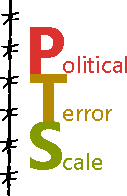
\includegraphics[scale=1]{PTS-Logo.pdf}\\}
\date{\vspace{6.5cm} \small{Updated: \today \\~\\~\\ \href{http://www.politicalterrorscale.org/}{http://www.politicalterrorscale.org/}}}
\maketitle

\pagenumbering{roman}

\chapter*{\vspace{3.5cm} License}

This document is released under the Creative Commons Attribution license CC BY-NC 4.0 -- \ccbync \\ \href{http://creativecommons.org/licenses/by-nc/4.0/}{http://creativecommons.org/licenses/by-nc/4.0/}\\~\\

\noindent\textbf{\large{Data and Citation:}}\\

\noindent The \PTS~dataset and this codebook can be found at \href{http://www.politicalterrorscale.org/}{http://www.politicalterrorscale.org/}. Please cite this codebook when appropriate. When using the \PTS~data, please cite:\\

\begin{quote}
Gibney, Mark, Linda Cornett, Reed Wood, Peter Haschke, and Daniel Arnon. 2015. The Political Terror Scale 1976-2016. Date Retrieved, from the Political Terror Scale website: http://www.politicalterrorscale.org/. 
\end{quote}
~\\~\\
\noindent\textbf{\large{Principal Investigators:}}\\

\noindent Mark Gibney \textit{(University of North Carolina, Asheville)}\\
\noindent Reed M. Wood \textit{(Arizona State University)}\\
\noindent Linda Cornett \textit{(University of North Carolina, Asheville)}\\
\noindent Peter Haschke \textit{(University of North Carolina, Asheville)}\\
\noindent Daniel Arnon \textit{(Emory University)}


\vspace{2.5cm}
\noindent If you have any questions, comments, and or concerns relating to this document, or require the \LaTeX~source code, please contact Peter Haschke (\href{mailto:phaschke@unca.edu} {phaschke@unca.edu}).

\clearpage

%%%%%%%%%%%%%%%%%%%%%%%%%%%
%%%%%     T.O.C.      %%%%%
%%%%%%%%%%%%%%%%%%%%%%%%%%%

\pagebreak

\thispagestyle{empty}

\tableofcontents

\pagebreak


%%%%%%%%%%%%%%%%%%%%%%%%%%%
%%%%%   Main Doc      %%%%%
%%%%%%%%%%%%%%%%%%%%%%%%%%%

%%%%%%%%%%%%
% CHAPTER  %
%%%%%%%%%%%%

\clearpage
\pagenumbering{arabic}
\chapter*{The Political Terror Scale (\PTS)}
\addcontentsline{toc}{chapter}{The Political Terror Scale (\PTS)}

\onehalfspacing

\section*{Introduction}
\addcontentsline{toc}{section}{Introduction}

This document describes the Political Terror Scale (\PTS) dataset, a data collection project housed by the Political Science Department at the University of North Carolina, Asheville. The dataset is described in detail in \citet{WoodGibney2010}. The \PTS~measures violations of physical integrity rights carried out by states or their agents -- covering some 200 countries or territories from 1976 to 2015. The dataset is available for download at: \href{http://www.politicalterrorscale.org/}{http://www.politicalterrorscale.org/}.

\section*{Definition of ``Political Terror''}
\addcontentsline{toc}{section}{Definition of ``Political Terror''}

The \PTS~seeks to measure \textit{political terror}. We define political terror as \textit{violations of basic human rights to the physical integrity of the person} by \textit{agents of the state}. It is important to note that political terror as defined by the \PTS~is not synonymous with \textit{terrorism} or the use of violence and intimidation in pursuit of political aims. The concept is also distinguishable from terrorism as a tactic or from criminal acts.

\subsection*{Violations of Physical Integrity}
\addcontentsline{toc}{subsection}{Violations of Physical Integrity}

Violations of physical integrity rights -- also referred to as \textit{violations of personal integrity or security} -- constitute the scope of violence that is captured by the \PTS. Violations of physical integrity rights include:

\begin{itemize}
  \item torture and cruel and unusual treatment and punishment;
  \item beatings, excessive use of force, brutality;
  \item rape and sexual violence;
  \item killings and unlawful use of deadly force;
  \item summary or extra-judicial executions;
  \item political assassinations and murder;
  \item political imprisonment, arbitrary arrest and detention;
  \item incommunicado and clandestine imprisonment and detention;
  \item forced disappearances;
  \item kidnappings, forced relocations and removal;
\end{itemize}

\noindent Not considered are corporal and capital punishment in the context of legal proceedings conforming to international standards.

\subsection*{Agents of the State}
\addcontentsline{toc}{subsection}{Agents of the State}

Physical integrity rights violations are only captured \textit{if} they are perpetrated, sanctioned, or ordered by \textit{agents of the state}. Domestic, societal, or criminal violence, or violence ascribed to insurgent groups or criminal syndicates are not considered. Examples of state agents or actors acting on the behest, or on the authority or with implicit consent of agents of the state, include:

\begin{itemize}
  \item police, law enforcement, guards, and security personnel 
  \item military and paramilitary organizations
  \item executives and members of executive agencies and bureaucracies
  \item members of the criminal justice and penal systems (e.g. prison guards)
  \item intelligence agents
  \item militias
  \item death squads
  \item political parties and their organizations
  \item mercenaries and private military contractors
  \item foreign personnel such as peace-keepers supplementing domestic capacity
\end{itemize}

\noindent Identifying agents of the state and distinguishing them from non-state actors is often difficult. Where violations cannot be attributed to state agents, these violations are not coded. 

\subsection*{Motivations}
\addcontentsline{toc}{subsection}{Motivations}

It is important to note that the \PTS~does not exclude ``non-politically motivated violations'' of physical integrity rights by state agents. The \PTS~captures any violation of physical integrity rights by state agents, regardless of reasons or motivation for the violation. The assassination of a political challenger, for example, is counted the same way as the killing of a suspected criminal or a random by-stander. General police brutality, for instance, will be taken into account even in the absence of explicit repressive policies.\\  

\noindent As such, it is worth to point out that the \PTS~does not exclusively measure repression. Repression as understood in the literature is the use of violence and intimidation in pursuit of political aims \citep{Tilly1978,Goldstein1978,Gurr1986,Haschke2014}. The \PTS~captures the use of violence by state agents for any aim -- political, personal, or monetary.


\section*{Sources}
\addcontentsline{toc}{section}{Sources}

\section*{Unit of Observation}
\addcontentsline{toc}{section}{Unit of Observation}

\section*{Scaling}
\addcontentsline{toc}{section}{Scaling}

\subsection*{Intensity}
\addcontentsline{toc}{subsection}{Intensity}

\subsection*{Range}
\addcontentsline{toc}{subsection}{Range}

% ~\\~\\
% standards based\\
% unit of analysis\\


\chapter*{General and ID Variables}
\addcontentsline{toc}{chapter}{General and ID Variables}

\section*{\Variables{Country}}

Name of country or entity covered in human rights reports. In most cases names refer to independent states. Technically, the unit of analysis of the \PTS~ data is the \textit{report-year} and not the \textit{country-year}. As such, some entities covered are not independent states or UN members. Potentially controversial examples of ``non-states'' covered include: Western Sahara, Taiwan, Kosovo, the Occupied Territories, Gaza, the European Union, and Puerto Rico.

\section*{\Variables{Country\_OLD}}

Name of country or entity covered in human rights reports as used in previous data releases. 

\section*{\Variables{Year}}
Year of observation. Note that this is not the year of publication but the year of events covered in reports. For example, the ``World Report 2016'' published by Human Rights Watch in 2016 covers events that took place in 2015.  

\section*{\Variables{COW\_Code\_A}}

The Correlates of War Project (CoW) alphabetic country codes. Details can be found here: \href{http://www.correlatesofwar.org/data-sets/cow-country-codes}{http://www. correlatesofwar.org/data-sets/cow-country-codes}.

\section*{\Variables{COW\_Code\_N}}

The Correlates of War Project (CoW) numeric country codes.

\section*{\Variables{WordBank\_Code\_A}}

World Bank three letter country codes (ISO 3166-1 alpha-3). Details can be found here: \href{http://data.worldbank.org/developers/api-overview/country-queries}{http://data. worldbank.org/developers/api-overview/country-queries}.

\section*{\Variables{UN\_Code\_N}}

United Nation three digit numeric country codes (ISO 3166-1 numeric-3). Details can be found here: \href{http://unstats.un.org/unsd/methods/m49/m49alpha.htm}{http://unstats .un.org/unsd/methods/m49/m49alpha.htm}.

\section*{\Variables{GW\_Code\_A}}
Gleditsch and Ward \citeyearpar{GleditschWard1999} alphabetic country codes. Details can be found here: \href{http://privatewww.essex.ac.uk/~ksg/data/iisyst_casedesc.pdf}{http://privatewww. essex.ac.uk/$\sim$ksg/data/iisyst\_casedesc.pdf}.

\section*{\Variables{GW\_Code\_N}}

Gleditsch and Ward \citeyearpar{GleditschWard1999} numeric country codes.

\section*{\Variables{Region}}

OECD region identifier. 

\begin{itemize}
  \item eap -- East Asia and Pacific
  \item eca -- Europe and Central Asia
  \item lac -- Latin America and Caribbean
  \item mena -- Middle East and North Africa
  \item na -- North America
  \item sa -- South Asia
  \item ssa -- Sub-Saharan Africa
\end{itemize}


\chapter*{\PTS~Variables}
\addcontentsline{toc}{chapter}{\PTS~Variables}

\section*{\Variables{PTS\_A} ~~ PTS Amnesty International (PTS-A)}

\blindtext

\section*{\Variables{PTS\_S} ~~ PTS State Department (PTS-S)}

\blindtext

\section*{\Variables{PTS\_H} ~~ PTS Human Rights Watch (PTS-H)}

\blindtext

\chapter*{New \PTS~Variables}
\addcontentsline{toc}{chapter}{New \PTS~Variables}

\section*{\Variables{Exists\_Beta}}\blindtext
\section*{\Variables{NoReport\_A\_Beta}}\blindtext
\section*{\Variables{NoReport\_H\_Beta}}\blindtext
\section*{\Variables{NoReport\_S\_Beta}}\blindtext
\section*{\Variables{NoPTS\_A\_Beta}}\blindtext
\section*{\Variables{NoPTS\_H\_Beta}}\blindtext
\section*{\Variables{NoPTS\_S\_Beta}}\blindtext



\clearpage
\addcontentsline{toc}{chapter}{Index of Variables}
\printindex
\clearpage

\addcontentsline{toc}{chapter}{Bibliography}
\normalsize
 \bibliography{PTS.bib}
   \bibliographystyle{apsr}

\end{document}